\section{Proposed ChatBot}
%
\subsection{DataModel}
\subsubsection{Chosen technology}
\subsubsection{Structure}
\paragraph{Vertexes}
\paragraph{Edges}
%
\subsection{User Interface}
\subsubsection{Chosen technology}
\label{subs:Technology}

\paragraph{State of the Art}
\label{par:SotA}
Obviously, this is a Python project, because the point of the course is to discover NLP and Text-mining by using NLTK.
So, we decided to naturally go and try our way in Python to get an interface for our chat-bot.
In the litterature, there are two main approaches for doing that :
\begin{itemize}
    \item Interfacing our bot on an IRC server, and using an IRC client as a User Interface.
    \item Developing our own interface.
\end{itemize}
As we wanted the user to be able to rate our bot's answers, the first solution was never really an option.
An IRC (or so) client's interface doesn't give us room for non-textual interaction, and it is something which was important for us.
The second solution, developing our own interface, is quite easy in Python, as long as you have more than just notions in web development.
We explored two Python frameworks, \textit{Django} and \textit{Flask}.
\textit{Django} is obviously way too dense and heavy for our needs, so we tried our best with Flask.
Considering that the user interface is not a very important component of our application, we decided that Flask was also a waste of time for us, and that we should do what we could already do.

\paragraph{Shiny}
\label{par:Shiny}
Therefore we decided to propose a R user interface.
R is, like Python, an open-source interpreted language, but it is specialized in Data Mining.
Its main IDE, RStudio, proposes a package for building easily interactive web interfaces.

\paragraph{Interfacing R with Python}
\label{par:rPython}
The point of the project still being to develop a chat-bot based on NLP and text-mining (in Python, using NLTK), we figured out a way of connecting both, and built APIs to do it easily.
Our app is called through R interpreter, which launches the User Interface. Then, the R server calls for the answering API, which eventually calls Python answering engine.

\newpage
\subsubsection{Result}
\label{subs:Result}

\begin{figure}[!h]
\begin{center}
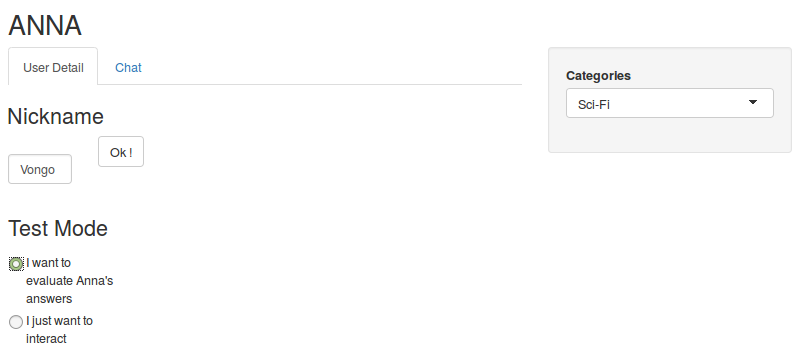
\includegraphics[width=0.70\textwidth]{./img/AnnaLoginUI.png}
\end{center}
\caption{LogIn Interface, where you can also decide whether you want to evaluate Anna's answers.}
\label{fig:AnnaLoginUI}
\end{figure}

\begin{figure}[!h]
\begin{center}
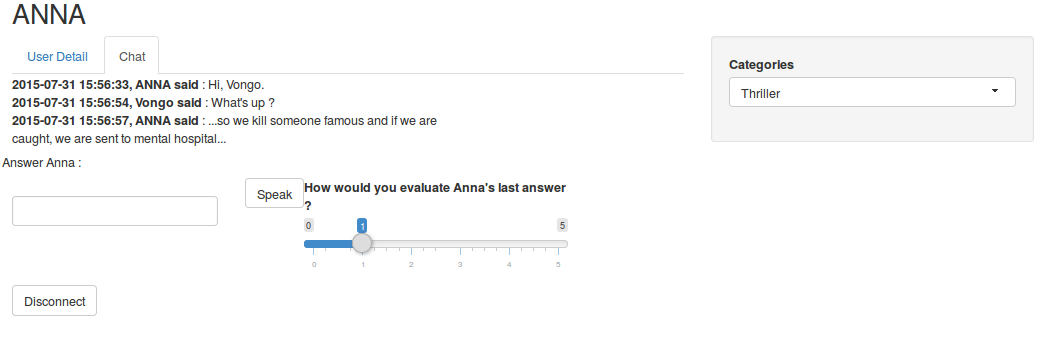
\includegraphics[width=0.80\textwidth]{./img/AnnaChatUI.png}
\end{center}
\caption{Chat Interface : a simple chat session.}
\label{fig:AnnaChatUI}
\end{figure}

\\subsection{Architecture}
\label{sub:Architecture}


%
\subsection{Anna's answers}
\subsubsection{Version 1 : Random answers}
\subsubsection{Version 2 : Determined SentenceType}
\subsubsection{Version 3 : Determined movie genre}
